% LLNCStmpl.tex
% Template file to use for LLNCS papers prepared in LaTeX
%websites for more information: http://www.springer.com
%http://www.springer.com/lncs
\documentclass{llncs}

\usepackage{graphicx}
\usepackage{float}
\usepackage{hyperref}

\begin{document}
\title{Linux client with WiFi and LTE}
\subtitle{Project report}
\author{Pascal Maissen, Jovana Micic, Noe Wysshaar} 
\institute{University of Bern\\  \email {pascal.maissen@unifr.ch, jovana.micic@students.unibe.ch, noemathieu.wysshaar@unifr.ch} }
\maketitle

%Maximum 2 pages about the theoretical basics of the experiment.
\section{Protocol Introduction}
The task of this project is study of Dynamic Adaptive Streaming over HTTP video delivery in a mobile scenario using WiFi and Long Term Evolution (LTE). Case scenario is that the user is connected through LTE, but periodically gets the internet access through WiFi. The main goal of this project is to evaluate the quality gain in the parallel LTE/WiFi video transmission in comparison to a single LTE transmission using multi-path TCP (MPTCP).

In order to achieve parallel connection of LTE and WiFi we have to use MPTCP. Multi-path TCP is a  recent attempt  to handle simultaneous use of multiple paths at the transport layer \cite{MPTCP}. The core idea of MPTCP is to define a way to build a connection between two hosts and not between two interfaces (as standard TCP does). MPTCP represents the evolution of TCP protocol and it works in all networks where TCP works.  Benefits of MPTCP include better resource utilization, better throughput and smoother reaction to failures. Using MPTCP dramatically improves Quality of Experience of video streaming. 

\begin{figure}[H]
\centering
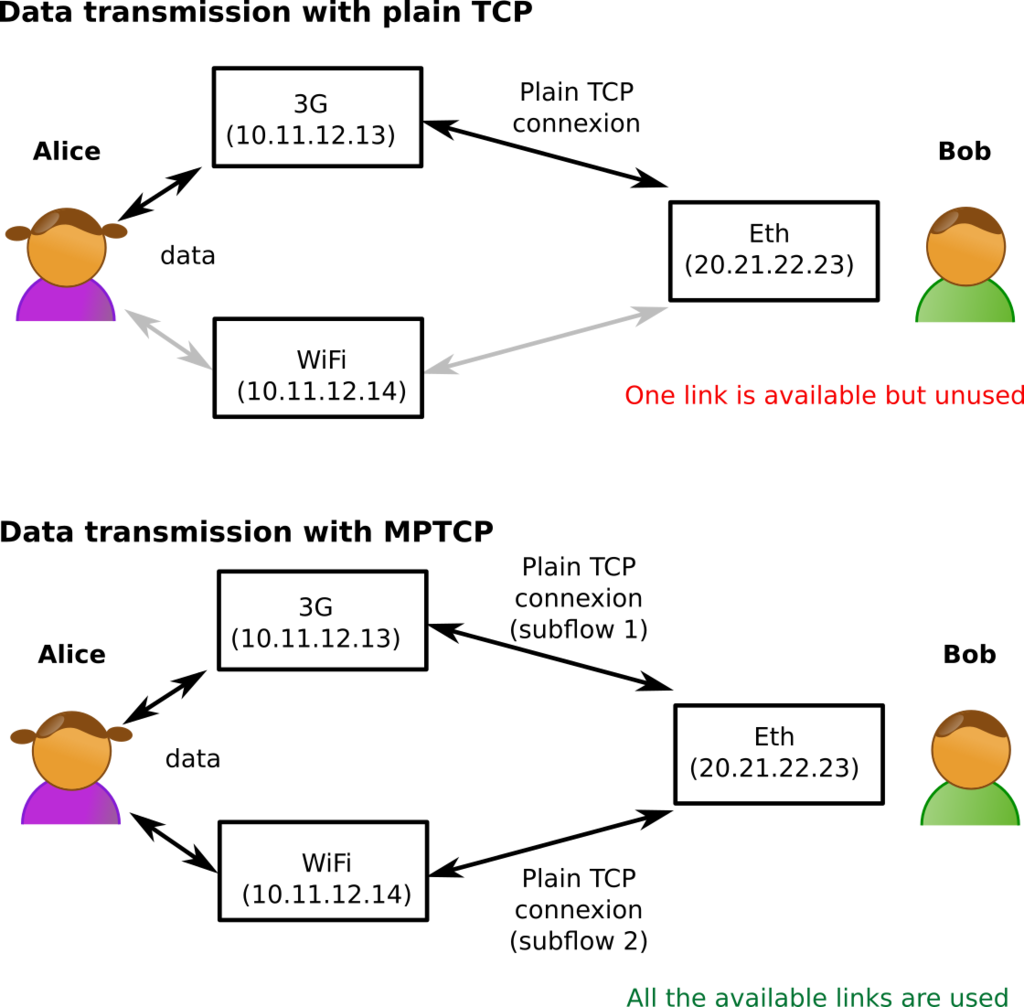
\includegraphics[width=0.5\textwidth]{mptcp.png}
\caption{\label{fig:mptcp} Difference between TCP and MPTCP}
\end{figure}

In the figure \ref{fig:mptcp} is presented graphic explaining the difference between TCP and MPTCP.  For instance, Alice has a smartphone with 3G and WiFi interfaces and Bob has a computer with an Ethernet interface. In standard TCP, the connection should be established between two IP addresses. An application can only create one TCP connection through a single link. MPTCP allows the connection to use several paths simultaneously. For this, MPTCP creates one TCP connection, subflow, over each path that needs to be used. So in the case from the figure \ref{fig:mptcp},  Alice can use both available links, 3G and WiFi at the same time.

In our project description it was required to use Dynamic Adaptive Streaming over HTTP (DASH). DASH is a streaming technique that enables high quality streaming of media content over the Internet \cite{DASH}. DASH works by breaking the content into a sequence of small HTTP-based file segments, each segment containing a short interval of playback time of content that is potentially many hours in duration, such as a movie or the live broadcast of a sports event. The content is made available at a variety of different bit rates, i.e., alternative segments encoded at different bit rates covering aligned short intervals of playback time. DASH client can adapt to changing network conditions and provide high quality playback with fewer stalls or re-buffering events. DASH should not be confused with a transport protocol, the transport protocol that DASH uses is TCP.

\begin{figure}[H]
\centering
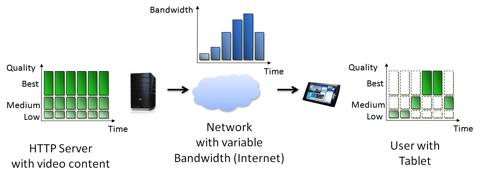
\includegraphics[width=1.0\textwidth]{DASH.png}
\caption{\label{fig:dash} Concept of Dynamic Adaptive Streaming over HTTP}
\end{figure}

In the figure \ref{fig:dash} is presented concept of DASH. This concept is consisting of the three parts. First part is HTTP server with video content of different qualities. Second part is network which has varying bandwidth conditions. Third part is user with device which selects appropriate segments for each timepoint. So the main advantage of using DASH is that is flexible, it dynamically adapts to current network conditions and it reuses existing Internet architecture.

%The experimental setup, the differences of the experimental series, the different parameters used.
\section{Experimental setup}
... 
\\
In our project we used Linux kernel implementation of MPTCP \cite{linuxMPTCP}. 
\\
...
\\
In the first part of our experiment we just tested throughput of the data without video streaming. We had two different scenarios:

\begin{enumerate}
\item{LTE and WiFi working in parallel. WiFi was turned off after 10 seconds and then turned on after 10 seconds.}
\item{WiFi was turned off and LTE was on. WiFi was turned on after 10 seconds.}
\end{enumerate}

In the second part of our experiment we wanted to test data throughput in a scenario when user is watching a video content from the Internet. As the video content we used a datasets  \cite{dataset} provided by Insititute for Information Technology from University in Klagenfurt, Austria. It contains already prepared DASH configured videos. As the player for the video streaming we used VLC player. VLC media player is a free and open-source, portable, cross-platform media player and streaming media server developed by the VideoLAN project. We used version 2.1.0 for Windows platform \cite{VLC}. 

%Analyze your data with respect to the aim of the experiment. Your task during the experiment is not just to measure and document your measurements, but to derive and present conclusions from your measurements. If there are some errors in the final results. Investigate and try to understand all types and sources of errors in all your measurements.
\section{Results and Analsys}
As it was mentioned in the previous section, for the first part of the project we measure data throughput for the two case scenarios. In the following text we will present results we got from this experiments.

\begin{figure}[H]
\centering
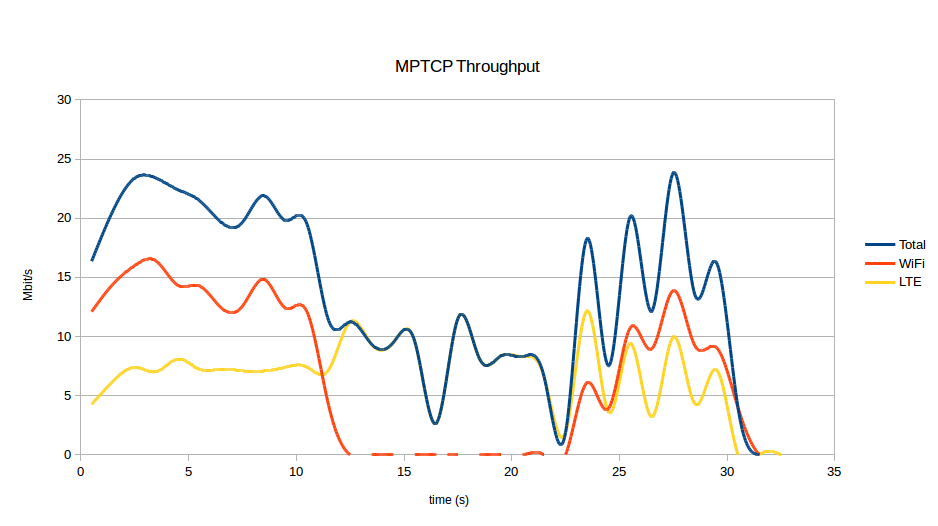
\includegraphics[width=1.0\textwidth]{result1.png}
\caption{\label{fig:r1} Graphic representing the MPTCP throughput when WiFi is turned off after 10 sec.}
\end{figure}

In the figure \ref{fig:r1} is presented throughput in the scenario when we have in parallel WiFi and LTE from the beginning of the experiment. After 10 seconds, we turned off WiFi. As we can see from the graphic, LTE continues to work but total throughput becomes lower and equal as LTE throughput. After 10 seconds, we had again turned WiFi on and it can be seen clearly on the figure that we have some WiFi throughput after 20 seconds. The maximal total throughput achieved in this scenario is around 24 Mbit/s.

\begin{figure}[H]
\centering
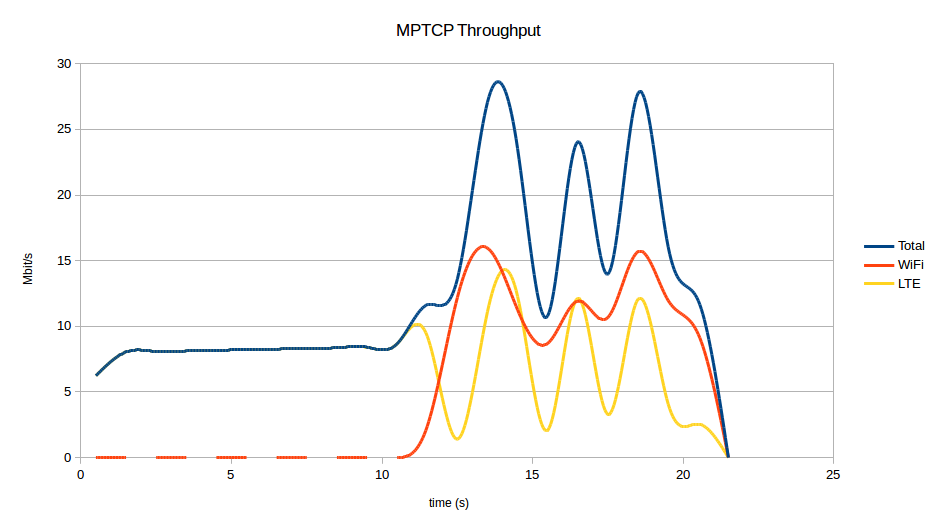
\includegraphics[width=1.0\textwidth]{result2.png}
\caption{\label{fig:r2} Graphic representing the MPTCP throughput when WiFi is turned on after 10 sec.}
\end{figure}

In the figure \ref{fig:r2} is presented throughput in the scenario when only LTE is turned on from the beginning of the experiment. After 10 seconds, WiFi is turned on. From the graphic we can see that there is increase of total throughput when WiFi is on. The maximal total throughput achieved in this scenario is around 28 Mbit/s.

The interesting observation from both graphics is that in the moment when the WiFi is again turned on, we have decrease of the LTE throughput. Reason for this could be specific MPTCP protocol implementation but we can not claim this with great certainty.

% @Pascal can you add few sentences about problems we had in first attempts? 

%Summarize and discuss your results with respect to the literature or your own scientific expectations. You should in particular discuss possible error sources and give a short judgment on the quality of the experimental setup (because you also learn to design the measurement setups). If needed, suggest how to improve the setups.
\section{Conclusions}
After running the several experiments of our setup, we can conclude that combination of Multipath TCP and DASH improves data throughput and Quality of Experience in video streaming as it was expected. We would like to mention that documentation and tutorials for setting up MPTCP Linux Kernel \cite{linuxMPTCP} are very poor and not very helpful. Because of that we are very thankful to Dr. Eryk Schiller for helping us with setting everything up. 


%The bibliography, done here without a bib file
%This is the old BibTeX style for use with llncs.cls
\bibliographystyle{splncs}
\begin{thebibliography}{1}
%add each reference in here like this:
\bibitem{MPTCP}
Barré, Sébastien. \emph{"Implementation and assessment of modern host-based multipath solutions." } Universite catholique de Louvain, Louvain-la-Neuve, Belgium (2011).

\bibitem{DASH}
Michalos, M. G., S. P. Kessanidis, and S. L. Nalmpantis. \emph{"Dynamic Adaptive Streaming over HTTP."} Journal of Engineering Science \& Technology Review 5.2 (2012).

\bibitem{linuxMPTCP}
C. Paasch, S. Barre, et al.. \emph{Multipath TCP in the Linux Kernel}. Available from \url{http://www.multipath-tcp.org}.

\bibitem{dataset}
\emph{DASH dataset}. Available from \url{www-itec.uni-klu.ac.at/ftp/datasets/mmsys12/}.

\bibitem{VLC}
\emph{VLC player}. Available from \url{download.videolan.org/pub/videolan/vlc/2.1.0/}.

\end{thebibliography}

\end{document}

